% !TeX spellcheck = da_DK
\input{../common/preamble.tex}

\title{Guide til lageret}
\author{Alexander Sommer \and Benjamin Wen \and Kristian Anton Hedegaard}
\date{\formatdate{27}{2}{2026}, opdateret \formatdate{9}{4}{2026}}

\begin{document}

\maketitle

Lager-ansvarlig er rollen der tidligere bestod af Indkøbsansvarlig og Indkøbsassistent. Ansvaret ligger i at sørge for at Fredagscaféen altid har fast inventar (fadøl, flaskeøl, sodavand hovedsagligt), og sørge for at sende pant og sådan noget tilbage igen.

\section{Fast Inventar}

Der er lavet fast sortiment liste på Drinx' hjemmeside, hvor man kan se alle de varer som er i sortiment for tiden. De(n) lageransvarlige kan opdatere denne liste, og tilpassse sortimentet.

Fast inventar er ikke nødvendigt fast. Det vil sige at det er op til den/de lager ansvarlig(e) hvad der er det faste inventar, men p.t. er det: 

\subsection{P-kælder}

\begin{itemize}
    \item Ceres Top 
    \item Tuborg Grøn
    \item Tuborg Classic 
    \item Odense Classic
    \item Høker Bajer (Hancock)
    \item Limfjordsporter (LFP)
    \item Hancock vand:
    \begin{itemize}
        \item Sports Cola 
        \item Cola og Sukkerfri Cola (evt. Hvid Cola)
        \item Appelsin og Appelsin Light
        \item Lemon 
        \item Sport (gennemsigtig)
        \item Mango/Passion
        \item Hindbær
        \item Ice-Cream Soda
        \item Orange Juice
        \item Tonic-Water
        \item Danskvand Blå
        \item Danskvand Citrus
    \end{itemize}
\end{itemize}

\subsection{Bag gitteret}

\begin{itemize}
    \item Diverse Breezer (6 slags)
    \item Smirnoff Ice 
    \item Pepsi 
    \item Pepsi Max
    \item Faxe Kondi
    \item Faxe Kondi Free
    \item Fire Energy Drink
    \item Cocio
    \item Caribia Ginger Beer
\end{itemize}

\subsection{Under trappen}

\begin{itemize}
    \item Absinthe
    \item 7 typer Sambuca
    \item Gin 
    \item Cuba Vodka 
    \item Cuba Caramel  
    \item Eristoff Red
    \item Rom (Hvid og gylden)
    \item Bacardi Coconut
    \item Captain Morgan Spiced Gold
    \item Tequila
    \item Gammel Dansk (lille mængde - rustur nostalgi)
    \item Jägermeister
    \item Bailey's
    \item Likor 43
    \item Ultrapres Beer Liquor 
    \item Minttu
    \item Pure Æble/Lakrids
    \item Diverse Små Shots
    \item Grenadine, Blå Curacao, Mango sirup
    \item Chips
    \item Bomb- og shotglas
\end{itemize}

Som eksempel på udskiftning har vi udfaset Kinley sodavand, for at strømline vores pant-setup, og indfaset Cocio + Likor 43 til kinderæg shots.

Chips kan købes hos Drinx eller i \foetex. Drinx har ``Kettle''-serien, som er billig nok i indkøb til at det giver mening. \foetex~har dog tit ``sjovere'' chips på tilbud.

\section{P-kælder}

I P-kælderen står vores fulde og tomme fustager samt det der står under sektionen P-kælder i sektionen ovenover. Derudover deler man plads med den/de specialølsansvarlig(e).\ 
Ved guidens skrivelse står alle kasser med øl/sodavand til højre, og fustager til venstre. Dette burde tages stilling til afhængig af hvordan lageret udvikler sig.
Vi er kommet frem til, at vi kan stable kasserne 6 høj, hvis den er 7 høj er det umuligt for lavere mennesker at tilgå dem (det er i forvejen svært med 6).
Det er også hernede CO$_2$ patroner står.


\section{Træburet}

I træburet står vores pant. Dette gælder både pantposer til dåser, og kasser med tomme flasker. Efter hver vagt stilles de herud. Det er en god idé at holde øje med status herude når man laver regulære checkups, for at sørge for det ikke hober sig op. Læs hvordan man skiller sig af med det i kapitlet Pant.

\section{Bag gitteret}

Her står vores Breezer, Smirnoff Ice og Fire Energy Drink. Vi kan også finde på at lægge vilkårlige kasser, såsom Ginger Ale og Kinley i hjørnet. Vi bruger øverste hylde til at opbevare kasser af Breezer/Ice/Fire, men ellers stilles det på hylderne. Her er det en god idé at koordinere med den specialølsansvarlige.

Her står også dåsesodavand, typisk på nederste hylde.

\section{Under trappen}

Alt det vi står for står på en hylde til højre når man går ind af døren. Her står alt vores spiritus og shots.

\section{Pant}

Vi har generelt tre forskellige former for pant, der kræver forskellige metoder at pante: 

\subsection{Kasser med standard ølflasker og cider-fustager}

Hver gang vi laver en bestilling fra Drinx, returnerer vi også pant, hvis der er nok til at fylde mindst en palle.
Dette gøres ved at man pakker en palle med øl- og Hancockkasser, samt cider-fustager, hvis der er nogen. En palle kan holde 30 kasser, i følgende opstilling:

\begin{figure}[H]
    \centering
    \includegraphics[width=0.5\linewidth]{palle_setup.png}
    \caption{Korrekt pakning af palle set fra oven}
    \label{fig:palle_setup}
\end{figure}

Denne skal stilles uden for porten til P-kælderen inde til højre. Husk at gøre plads til at der kan komme en levering også. Tomme cider-fustager fra Magners kan stilles øverst. Hele pallen skal pakkes sammen med wrap, der ligger i P-kælderen. 

\subsection{Tomme fustager fra Aarhus Bryghus}

Når man laver en bestilling ved Aarhus Bryghus kan man underrette dem om tomme fustager, som de så vil tage med når de leverer. Dette gælder også tomme CO$_2$ patroner.

\subsection{Dåser og diverse glasflasker}

Tomme dåser står i poser i træburet. På poserne er der en qr-kode som man kan scanne, hvorefter at de bliver tilføjet til at blive hentet som pant. Man skal bruge ``Vores Pant''-appen. Her skal man lige registreres først. Glasflasker, der ikke er normale glasflasker, vil blive lagt i glaskarret, som er i p-kælderen, og når det er fyldt kan man også scanne denne. Når karret er scannet vil Dansk Retur System komme og hente panten fra karret samt poserne med dåser. De kommer på et undisclosed tidspunkt på dagen, så der skal enten stå en person klar til at lukke dem ind, ellers skal man finde en palleløfter og stille det ud til dem ved siden af vejen. Hvis man stiller det ud til dem skal man stadig holde øje! Vi har fået stjålet pant før.

\section{Bestilling}

Cirka hver anden uge (nok hver uge i travle perioder) skal vi lave en bestilling. Det meste af inventaret bestilles via Drinx på en hjemmeside. Så stiller de det uden for porten til p-kælderen. Hertil er det meget fordelagtigt at finde en palleløfter, drift efterlader dem nogle gange ude. Man kunne overveje at lave en mere fast aftale med drift om at have palleløfteren tilgængelig.

Vores faste fustager, som er fra Aarhus Bryghus, bestiller vi via e-mail til Niels Buchwald. Det er også herfra vi får CO$_2$ patroner.
Når vi bestiller fra Drinx skal vi helst lave en bestilling for over 4.000 kroner for at få gratis levering. I kommentaren skal vi specificere hvor meget pant der skal hentes, og det er en god idé at specificere hvor panten/leveringsstedet er, det er sket før at de ikke kan finde det. Vi har en kontaktperson inde på Drinx, man kan forhandle priser med.
Aarhus Bryghus har adgang til vores lager, så ingen koordination behøves efter en bestilling. 

\section{Lidt mere fancy ting}
Af og til sker der flere ting end bare normal lagerpåfyldning. Dette er f.eks. at bestille ekstra ind til fester/events, være Aarhus Bryghus korrespondent hvis de får nogle seje specialøl (eller hvis den specialølsansvarlige vil have et kig) eller bare at cooke en ny drink eller lignende. Disse ting er svære at beskrive, men vær god til at snakke med resten af bestyrelsen, hvis der er noget der skal koordineres. For eksempel kunne formanden have godt overblik over hvad der skal bestilles ind til en fest, og om man skal cooke en sindssyg drink eller købe mere fancy øl fra Aarhus Bryghus.

Hvis flere spørgsmål skulle opstå, kan du hive fat i tidligere lageransvarlige: Benjamin eller Sommer.

\subsection{Husaftale på Spritfabrikken gennem Drinx}
Vi har en husaftale på Spritfabrikken gennem Drinx, hvor vi får 1 på 6 gratis på udvalgte varer. Umiddelbart bør det være indenfor hver linje på listen vi får 1 på 6. F.eks: 6 blandede Små Shots = 1 gratis. 6 Råstoff Salty Caramel = 1 gratis. 

Læs mere herunder, og kontakt Drinx hvis du har spørgsmål:
\begin{figure}[H]
    \centering
    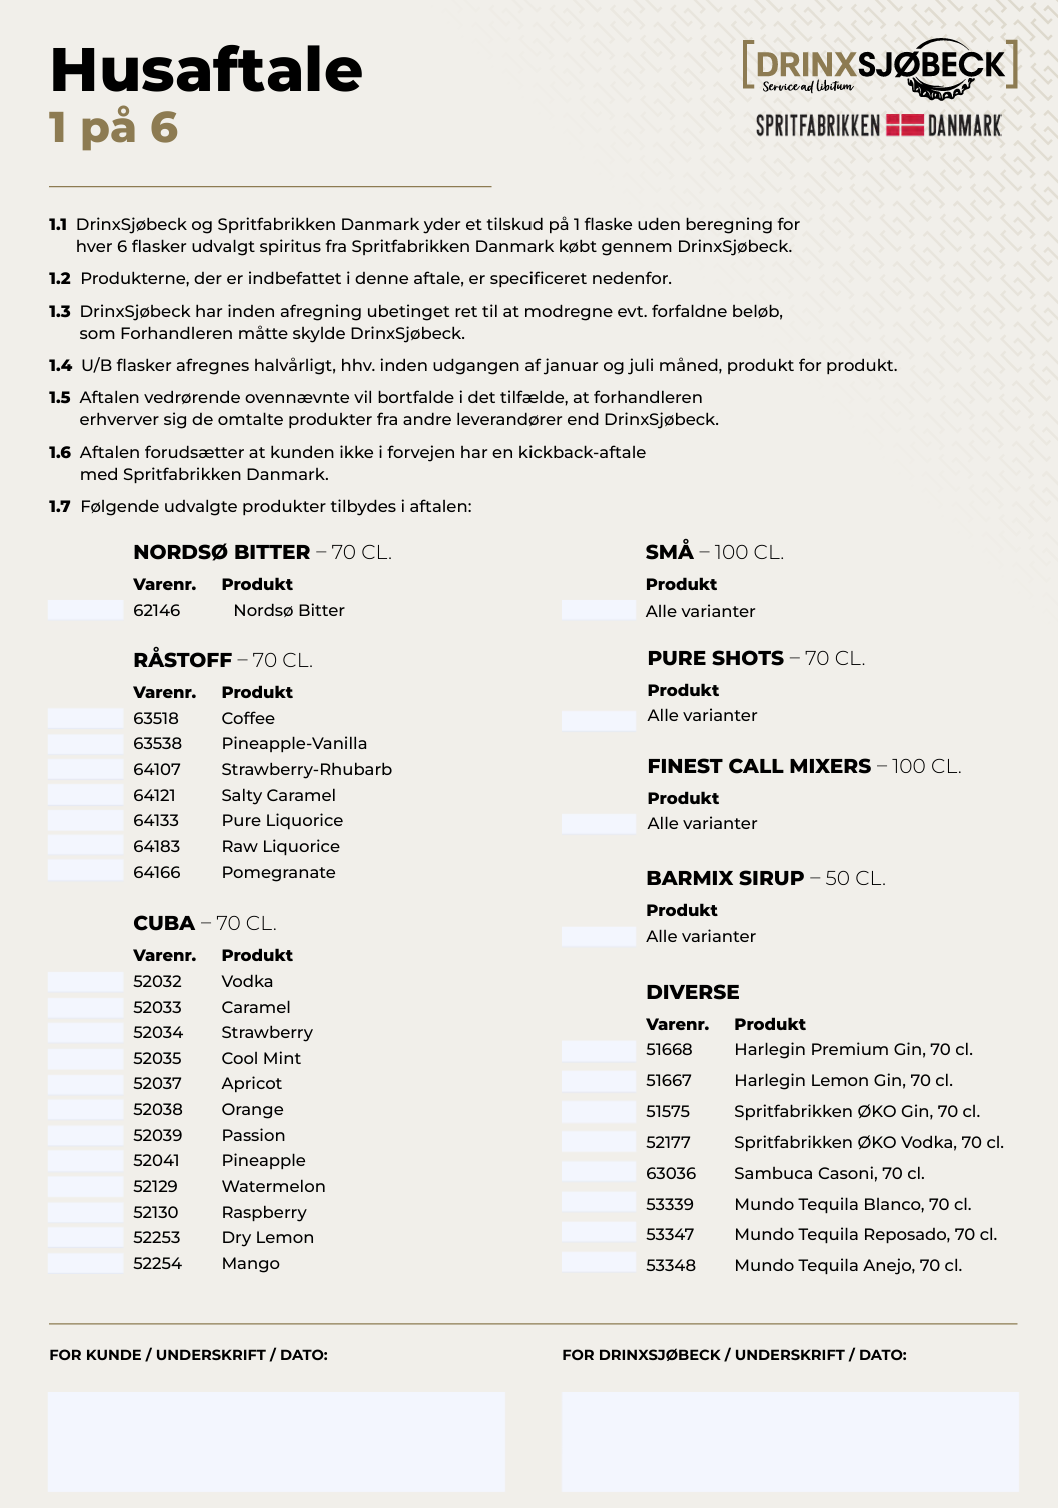
\includegraphics[width=0.6\linewidth]{husaftale.png}
    \caption{Husaftale på Spritfabrikken gennem Drinx}
    \label{fig:husaftale}
\end{figure}

\end{document}

%%% Local Variables:
%%% mode: latex
%%% TeX-master: t
%%% End:
